%%%%%%%%%%%%%%%%%%%%%%%%%%%%%%%%%%%%%%%%%%%%%%%%%%%%%%%%%%%%%%%%%
\begin{frame}[fragile]
\frametitle{\textbf{\textcolor{orange}{First definition}}}

\begin{Definition}
Let $n$ be a positive integer and $\omega \in R$.
\begin{itemize}
\item[\textbullet] $\omega$ is a \textcolor{violet}{$n$-th root of unity} if $\omega^{n} = 1$.
\item[\textbullet] $\omega$ is a \textcolor{violet}{primitive $n$-th root of unity} if :
\begin{itemize}
\item[(1)] $\omega^{n} = 1$.
\item[(2)] $\omega$ is a unit in $R$.
\item[(3)] $\forall t$ prime s.t. $t|n$, $\omega^{n/t} - 1$ is neither $0$ nor a $0$ divisor.
\end{itemize}
\end{itemize}
\end{Definition}

We now take $\omega \in R$ to be a primitive $n$-th root of unity.

\end{frame}

%%%%%%%%%%%%%%%%%%%%%%%%%%%%%%%%%%%%%%%%%%%%%%%%%%%%%%%%%%%%%%%%%
\begin{frame}[fragile]
\frametitle{\textbf{\textcolor{orange}{Discrete Fourier transform (DFT)}}}

\begin{Definition}
The $R$-linear map
$$\textcolor{darkgreen}{DFT_{\omega} : \begin{cases}
R^n &\rightarrow R^n \\
f &\mapsto (f(1), f(\omega), f(\omega^{2}),\dots,f(\omega^{n-1}))
\end{cases}}$$
which evaluates a polynomial at the powers of $\omega$ is called the \textcolor{red}{\textbf{Discrete Fourier Transform (DFT)}}.
\end{Definition}

\begin{prop}[consequence of the Lagrange's theorem]
The $R$-linear map $DFT_{\omega}$ is an isomorphism.
\end{prop}

Then we can represent a polynomial $f$ by the \textit{DFT} representation with $\omega$ determined in our code.

\end{frame}
%%%%%%%%%%%%%%%%%%%%%%%%%%%%%%%%%%%%%%%%%%%%%%%%%%%%%%%%%%%%%%%%%

%%%%%%%%%%%%%%%%%%%%%%%%%%%%%%%%%%%%%%%%%%%%%%%%%%%%%%%%%%%%%%%%%
\begin{frame}[fragile]
\frametitle{\textbf{\textcolor{orange}{Convolution}}}

\begin{Definition}
The \textcolor{violet}{\textbf{convolution}} w.r.t. $n$ of $f = \sum_{0\leq i < n} f_i\,x^i$ and $g = \sum_{0\leq i < n} g_i\,x^i$ in $R[x]$ is $h = f*g = \sum_{0\leq k < n}h_k\, x^k$ s.t.
$$\textcolor{darkgreen}{\forall k \in \mbox{\textlbrackdbl} 0, n-1\mbox{\textrbrackdbl},\; h_k = \sum_{i+j\equiv k \mod n}f_i\,g_j}.$$
\end{Definition}

\begin{block}{}
One can prove that $\textcolor{violet}{fg = f*g \mod (x^n-1)}$.
\end{block}

\begin{Lemma}[DFT product amounts to a scalar product]
For $f,g \in R[x]$ univariate polynomials of degree less than $n$ we have 
$$\textcolor{red}{DFT_{\omega}(f * g) = DFT_{\omega}(f)DFT_{\omega}(g)}.$$
\end{Lemma}


\end{frame}
%%%%%%%%%%%%%%%%%%%%%%%%%%%%%%%%%%%%%%%%%%%%%%%%%%%%%%%%%%%%%%%%%

%%%%%%%%%%%%%%%%%%%%%%%%%%%%%%%%%%%%%%%%%%%%%%%%%%%%%%%%%%%%%%%%%
\begin{frame}[fragile]
\frametitle{\textbf{\textcolor{orange}{FFT Maping}}}

\begin{Definition}
The \textcolor{red}{\textbf{Fast Fourier Transform (FFT)}} is an efficient algorithm to compute \textit{DFT} and its inverse. 
\end{Definition}

We use the \textcolor{violet}{Cooley-Tukey} algorithm following a \textit{D{\&}C} strategy.
\begin{center}
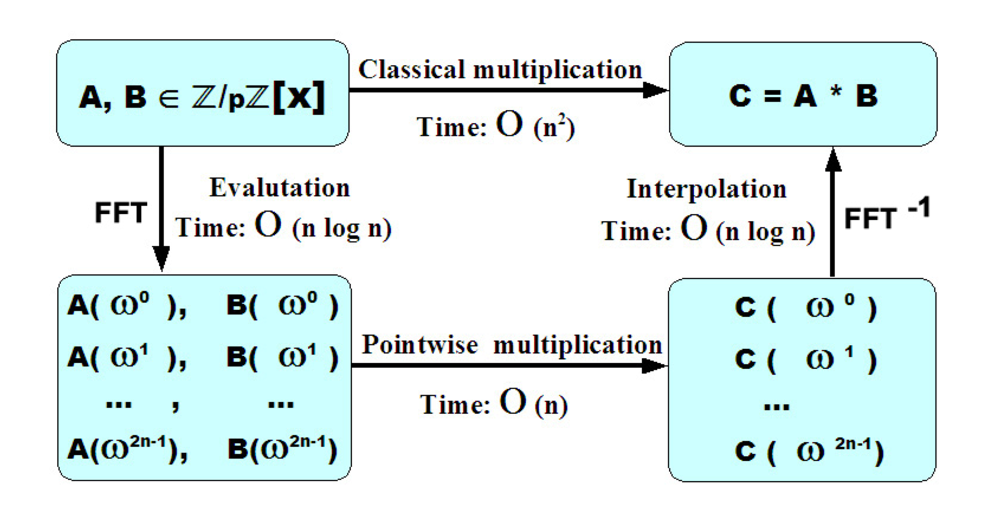
\includegraphics[scale = 0.2]{FFT.png}\\
\small\textbf{FFT-based univariate polynomial multiplication over $\mathbb{Z}/p\mathbb{Z}$}\\
\end{center}

\end{frame}
%%%%%%%%%%%%%%%%%%%%%%%%%%%%%%%%%%%%%%%%%%%%%%%%%%%%%%%%%%%%%%%%%
